\section{Show me music}
Dive into a multitude of topics that visualize the complex interrelations of melody, harmony and mathematics. Each of the animations looks at a certain musical piece or pattern from a special mathematical viewpoint. Aspects of symmetry, both in time and space help to understand musical ideas.

\begin{figure}[!h]
\centering
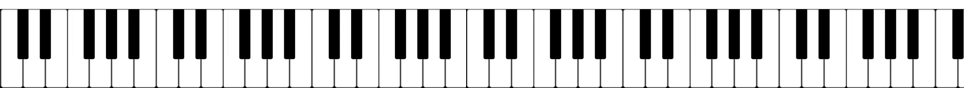
\includegraphics[width=\textwidth]{ShowMeMusic_1}
\end{figure}

\subsection{Spiral Tone Space}
The keys on a piano form a pretty regular pattern. Within every group of seven white keys the pattern of black and white keys repeats exactly. If you play the piano and shift your fingers up to the eighth white note on the right the music will sound almost exactly the same... just performed one octave higher. A nice way to express this fact mathematically is to arrange the tones in a spiral such that each full turn corresponds exactly to one octave.

\begin{figure}[h]
\centering
\begin{subfigure}{0.45\textwidth}
\centering
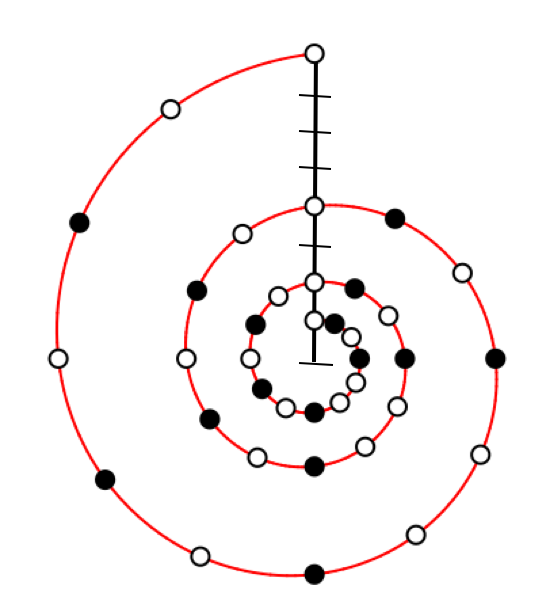
\includegraphics[height=4cm]{ShowMeMusic_2}
\end{subfigure}
\begin{subfigure}{0.45\textwidth}
\centering
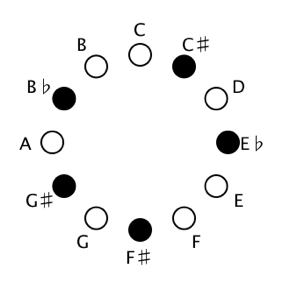
\includegraphics[height=4cm]{ShowMeMusic_3}
\end{subfigure}
\end{figure}


\paragraph{The Music:} The concept of an octave is close to omnipresent in music. Even throughout different cultures. Playing a tune one octave higher means essentially doubling all frequencies, and by this it is closely related to the overtone series. A piano usually covers a bit more than 7 octaves. The human singing voice covers usually around two octaves.

\paragraph{The Maths:} The picture above illustrates a sequence of three octaves mapped to a logarithmic spiral. Low tones are closer to the center of the spiral. It starts with a C and spirals clockwise to higher and higher notes. In order to keep track, the black and white pattern of the piano keys is used. The scaling of the spiral is chosen in a way that one full term corresponds to an octave and that the distance of any point to the center is proportional to its frequency. Thus along the vertical black ray you see four different ``C'' notes. Each of the twelve rays corresponds to one of the tones in our twelve-tone-system. Depending on the context it is often also reasonable not to distinguish between the same notes in different octaves, this leads to so called circular tone space.

\paragraph{The Exhibit:} The exhibit visualizes tones of well known tunes in the spiral tone space. Scaling parameters of the spiral are chosen slightly differently to squeeze in more octaves. Predominant notes (in circular tone space) are automatically detected and the corresponding tone class is highlighted. By this you can follow the dominating notes in a tune. Enjoy hearing and seeing music. Even watching well known tunes this way will reveal several hidden patterns and make the composition more transparent.

\subsection{Space of Three-Note Chords}
Sometimes surprising structures emerge if one studies objects from a standpoint that does not only look at one object but at many of them and their mutual relations. For instance, considering all possibilities to play a chord consisting of three notes is a surprisingly rich geometric object. For this let us ignore the octave information (and therefore for instance treat all C notes equally). The picture shows that space. Each point corresponds to exactly one possible chord. It turns out that this space forms a triangular prism filled with all together 364 possible chords. Each such point corresponds to a selection of three notes. The three vertical edges correspond to situations where all three notes are identical (maximally close together notes). The central axis of white dots corresponds to chords such as C-E-G$\sharp$ (stacked thirds, with maximally spread notes).

\begin{figure}[h]
\centering
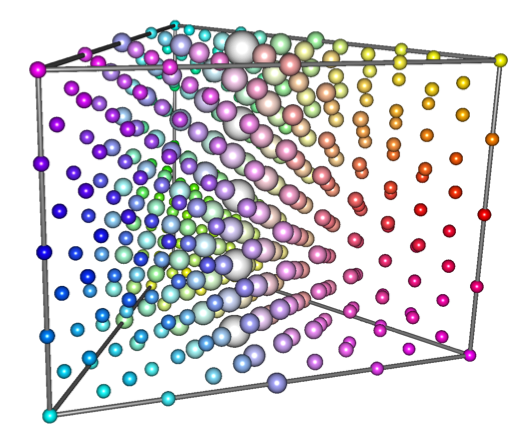
\includegraphics[width=0.6\textwidth]{ShowMeMusic_4}
\end{figure}

Chords that are close to each other in that space differ by a halftone step. Making small changes from one chord to another (by halftone step movements) means wandering around in that structure. Fixing two notes of a chord and changing the other in halftone steps results in a linear path in the inside of the prism. The quadrangular sides of the prism structure act like walls or mirrors at which the path bounces of. The top and the bottom of the prism have to be considered identified with a 120\textdegree twist. Hence leaving the structure on the top wormholes you and brings you back to the bottom of the figure.

\begin{wrapfigure}[18]{l}{0.35\textwidth}
\centering
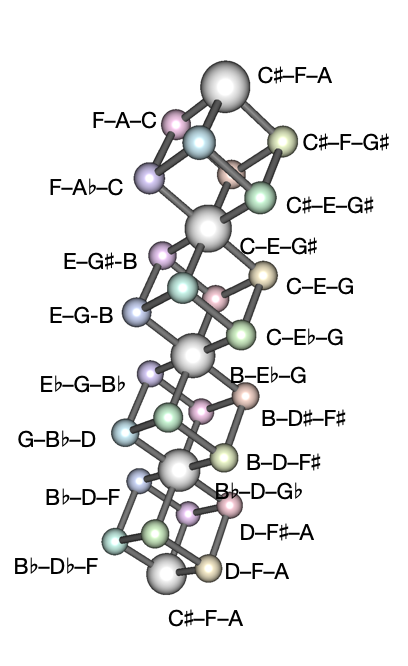
\includegraphics[width=0.34\textwidth]{ShowMeMusic_6}
\end{wrapfigure}
\paragraph{The Music:} This 3D structure encodes a lot of classical music theory. For instance at a distance of 1 to the central axis you can find all major and minor chords. In the picture below several chords are labeled. Classical chord progressions typically correspond to nice walks through this structure.

\paragraph{The Math}: This image has many deep relations to symmetry theory. The fact that the quadrangular faces act like mirrors and the top and bottom are identified makes this prism to be a fundamental cell of a 3-dimensional symmetric object in which infinitely many of such prisms fill the entire space. Just like a three dimensional symmetric wallpaper pattern. Considering the space of chords in such a general way is a relatively new field of research mainly driven by Princeton professor Dmitri Tymoczko.\\

\paragraph{The Exhibit:} The exhibit allows you to navigate in the space of such chords. The big red ball indicates the current position. A random arpeggio with the selected chord is played. Move the tones, listen to the chords and create your own musical progressions!

\begin{figure}[h]
\centering
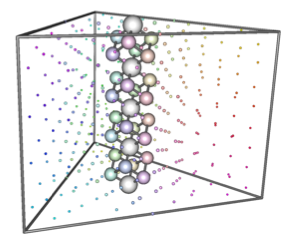
\includegraphics[width=0.5\textwidth]{ShowMeMusic_5}
\end{figure}


\subsection{Pachelbels Canon in D and Pachelballs}
Pachelbel's Canon in D is perhaps one of the most well known pieces of classical music. Despite the fact that it had already been composed around 1690 (most probably before Bach's works) it sounds amazingly fresh and modern. It follows a very simple but very impressive chord scheme that even today forms the basis of many well known Pop, Folk, Country, and Jazz Pieces as diverse as April Lavigne's Skater Boy, Bob Marley's No Woman No Cry or The Beatle's Let it be.

\paragraph{The Math:} A canon is repetition and repetition is symmetry. In a certain sense a canon is symmetry in time. The same pattern repeats after a certain amount of time has elapsed. As a matter of fact, the Canon of Pachelbel is slightly different from many other canons since the musical pattern of each voice does not repeat after a while.

\paragraph{The Music:} The fact that the single voices do not repeat allows Pachelbel to create a progression of density in the canon (unlike many other canons). Pachelbel composes with many tricky twists both rhythmically and melodically. Patterns that form the leading voice at one moment become the accompanying voice a few moments later.

\paragraph{The Exhibit:} Two of our exhibits are based on Pachelbel's Canon. One of them visualizes the entire piece and emphasizes the fact that all three voices play exactly the same score with a shift in time, the other exhibit (Pachelballs) is a game. Based on Pachelbel's chord pattern you can create soothing physics driven chimes.

%Pachelbel’s canon consists in a repeating chord progression, namely, a repeating cycle of the following 8 chords,
%Ab, Eb, Fm, Cm, Db, Ab, Db, Eb.
%Each chord is a set of three different notes, but here we double each note on two octaves, so each chord here corresponds to 6 notes. Precisely,
%Ab = [Eb4,Ab4,C5 ,Eb5,Ab5,C6 ]
%Eb = [Eb4,G4 ,Bb4,Eb5,G5 ,Bb5]
%Fm = [C4 ,F4 ,Ab4,C5 ,F5 ,Bb5]
%Cm = [C4 ,Eb4,G4 ,C5 ,Eb5,G5 ]
%Db = [Ab3,Db4,F4 ,Ab4,Db5,F5 ]
%Ab = [Ab3,C4 ,Eb4,Ab4,C5 ,Eb5]
%Db = [Ab3,Db4,F4 ,Ab4,Db5,F5 ]
%Eb = [Bb3,Eb4,G4 ,Bb4,Eb5,G5 ]
%At each given moment, there is one selected chord. The six bars of the game are connected to the six notes of that chord. When a ball bounces on a bar, it plays the note associated to that bar.
%With a fixed rhythm, the selected chord shifts to the next one and the bars are reassigned. Each chord shift happens every two ball shots.


\begin{figure}[t]
\centering
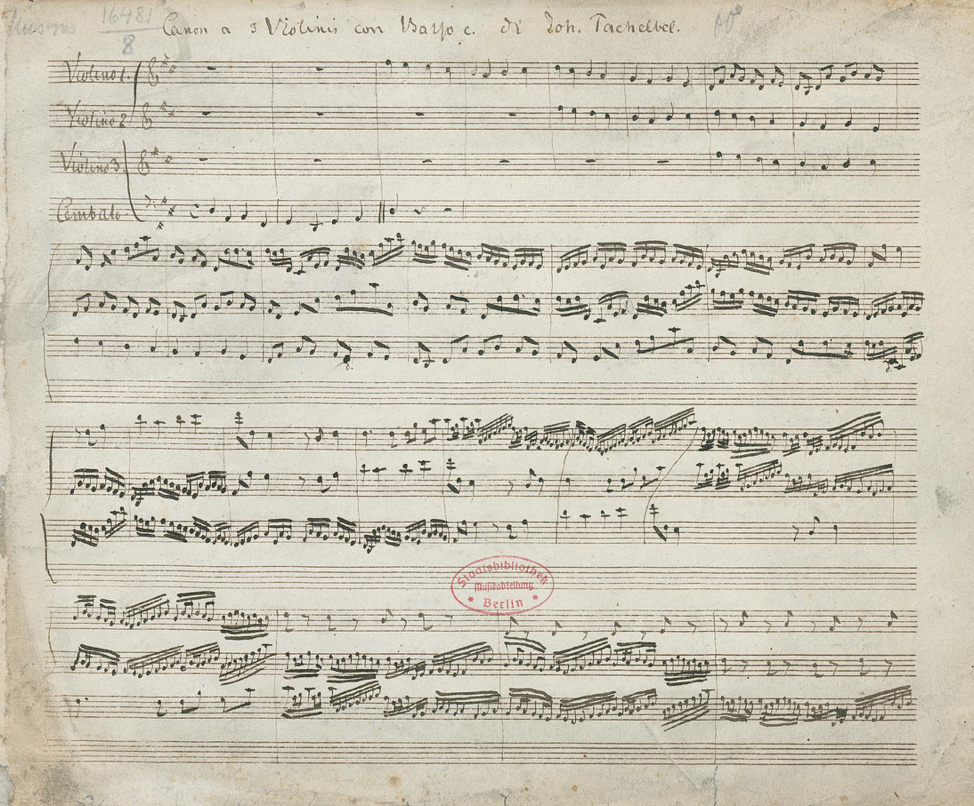
\includegraphics[width=0.7\textwidth]{ShowMeMusic_7}
\end{figure}


\subsection{Mozart's Musical Dice Game}
Some years after Mozarts death a musical dice game was published that is attributed to Mozart and most probably actually is his invention. In modern terms it might be called a randomized music generator. The game allows for the creation of a well sounding minuet that (with close to certain probability) was never played before. For this, Mozart presents a score with numbered measures. Along with the score comes a table that for each measure in the final waltz has a column of possible measures that can be used as a fill-in. Which fill-in is actually used for each measure is determined by throwing two dice, summing up their values and selecting the corresponding row for each measure. Amazingly, every waltz created in this way has a very authentic sounding Mozart feel to it.

\paragraph{The Music:} How did he do it? At a first glance, many people are amazed by well sounding music generated by a simple random procedure. At a second glance, this is not very surprising. The main musical content on a conceptual level is determined more by the underlying harmony progression than by the concrete melodic lines of a tune. For a given harmony there are many melodic ways to express the same idea. What Mozart does is to simply offer 11 ``equivalent'' choices for each measure. It is like replacing the sentence ``Wow, the bunny looks nice'' by ``Yeah, the rabbit is beautiful''. This is the reason why each of the minuets created in this game sounds more or less the same.

\begin{wrapfigure}[22]{r}{0.4\textwidth}
\centering
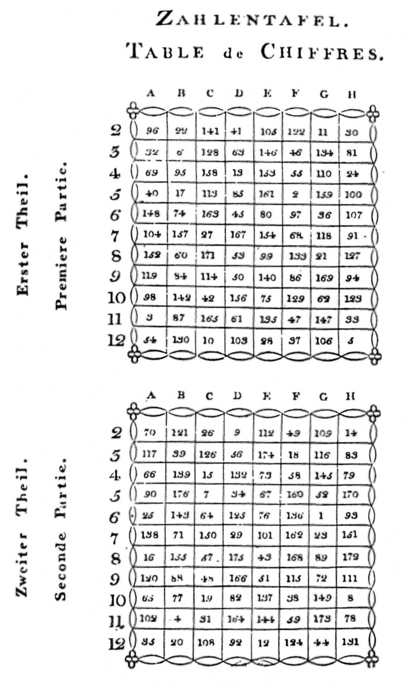
\includegraphics[width=0.4\textwidth]{ShowMeMusic_8}
\end{wrapfigure}

\paragraph{The Math:} The first and most obvious question is how many possible pieces of music, can there be created from Mozart's Dice Game? The waltz consists of two parts. Each of them consisting of eight bars. For each bar there are 11 choices which, with a little elementary combinatorics, makes an astronomic number of $11^{16} = 45 949 729 863 572 161$ possibilities. Listening to all of them would require around 60 billion years. Trust me, you would be pretty bored by then.

There is also a slightly subtler mathematical point to the game. The distribution of chosen measures will not be an equal distribution. Since for each bar the chosen possibilities are determined by the sum of two dice there is a bias toward the numbers in the middle rows. There are all in all $6\times 6=36$ possible outcomes of throwing the dice. Only one of them, 1+1 = 2, creates the number two, but six of them create the number 7 = 1+6 = 2+5 = 3+4 = 4+3 = 5+2 = 6+1.

\paragraph{The Exhibit:} You want your very individual never heard before Mozart piece. Just press the play button and enjoy.

\subsection{Shepard Tone}

\begin{wrapfigure}[39]{l}{0.25\textwidth}
\centering
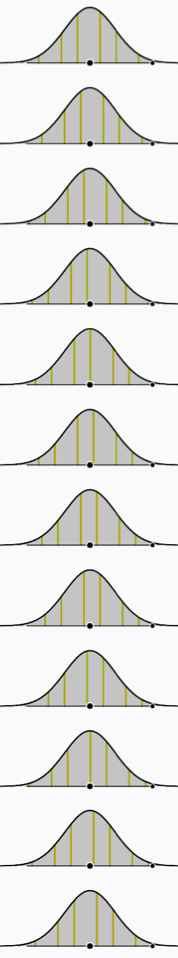
\includegraphics[height=0.9\textheight]{ShowMeMusic_9}
\end{wrapfigure}
Perception is a strange thing. Sometimes we hear or see things that are not really there. There is a phenomenal acoustic illusion that creates the effect of an ever rising or ever falling tone. Similar in concept to one of these Escher staircases that seem to ascend in every step, but actually just go in circles.

The illusion is generated in the following way: One defines a frequency window; ideally with smooth boundaries. This can be done by for example using a Gaussian bell curve. Within this window all overtones of a certain spectrum belonging to a tone are played. The amplitude of the different partial tones is determined by the window. Now the spectrum is shifted within the window (say in the direction of getting deeper). While deep overtones are faded out gradually new high notes enter the window. On average, the frequency remains the same. But each step sounds like a descending tone. This edict is called a Shepard tone.



\paragraph{The Music:} It is extremely difficult to play a convincing Shepard tone effect on a classical non-electronic instrument. It requires incredible control of the volume and intensity of the notes played. Nevertheless, it was used by modern composers in several musical pieces: Ligety's Piano etudes, or in the tension rich soundtrack by Hans Zimmer to the film Dunkirk, the end of Pink Floyd's Echoes or even in the soundtrack of the Super Mario Game when the protagonist is running an endless stair.

\paragraph{The Math:} A Creating Shepard tones requires a little fine tuning. Tones must enter and leave the spectrum almost without getting noticed. A good way to model this is to use a bell shaped Gaussian distribution that controls the intensity of the tones played. With this, even a very narrow range of frequencies produces a good effect. However, the broader and more overtone-rich the chosen spectrum is, the more convincing the effect. The picture shows the sonogram of a Shepard tone.

\paragraph{The Exhibit:} With our exhibit you can tune various parameters of the Shepard tone by simply changing the shape and position of the Gaussian curve involved. Explore how much freedom there is when creating this acoustic illusion.

\begin{figure}[h]
\centering
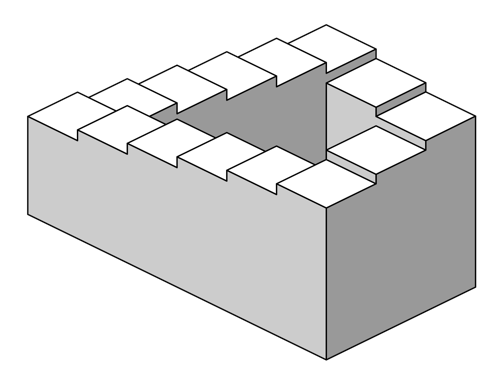
\includegraphics[width=0.5\textwidth]{ShowMeMusic_10}
\end{figure}
\strut
\vspace{6em}

\begin{sectcredits}
\item[Author of this exhibit:] Jürgen Richter-Gebert (Technical University of Munich)
\item[Acknowledgements:] Patrick Wilson and Aaron Montag (Sound Engine). Based on CindyJS.org
\item[Text:] Jürgen Richter-Gebert (TU Munich)
\end{sectcredits}
